\section{Przypadek Testowy 2 - Tabu Search - zależność PRD od liczby iteracji}
  \subsection{Cel:}
    W tej części zostaną ze sobą porównane PRD rozwiązania algorytmu Tabu Search w zależności od liczby iteracji.
    \subsection{Założenia:}
    Do badania tego przypadku zostały wykorzystane instancje grafów z paczki tsp. Dodatkowo maksymalna długość listy tabu równa 50, maksymalna liczba iteracji bez poprawy równa 200 oraz liczba sąsiadów równa 10\% wszystkich węzłów w grafie (zaokrąglona w dół). Ponad to dla każdej instancji ilość iteracji została ograniczona w zakresie od 100 do 1000 z iteracjią co 100;
  \subsection{Wyniki: }
    Ze względu na czytelność wszystkie wyniki są załączone w pliku \textbf{out\_test\_2.csv}.
  \subsection{Wykresy: }
    \begin{figure}[H]
      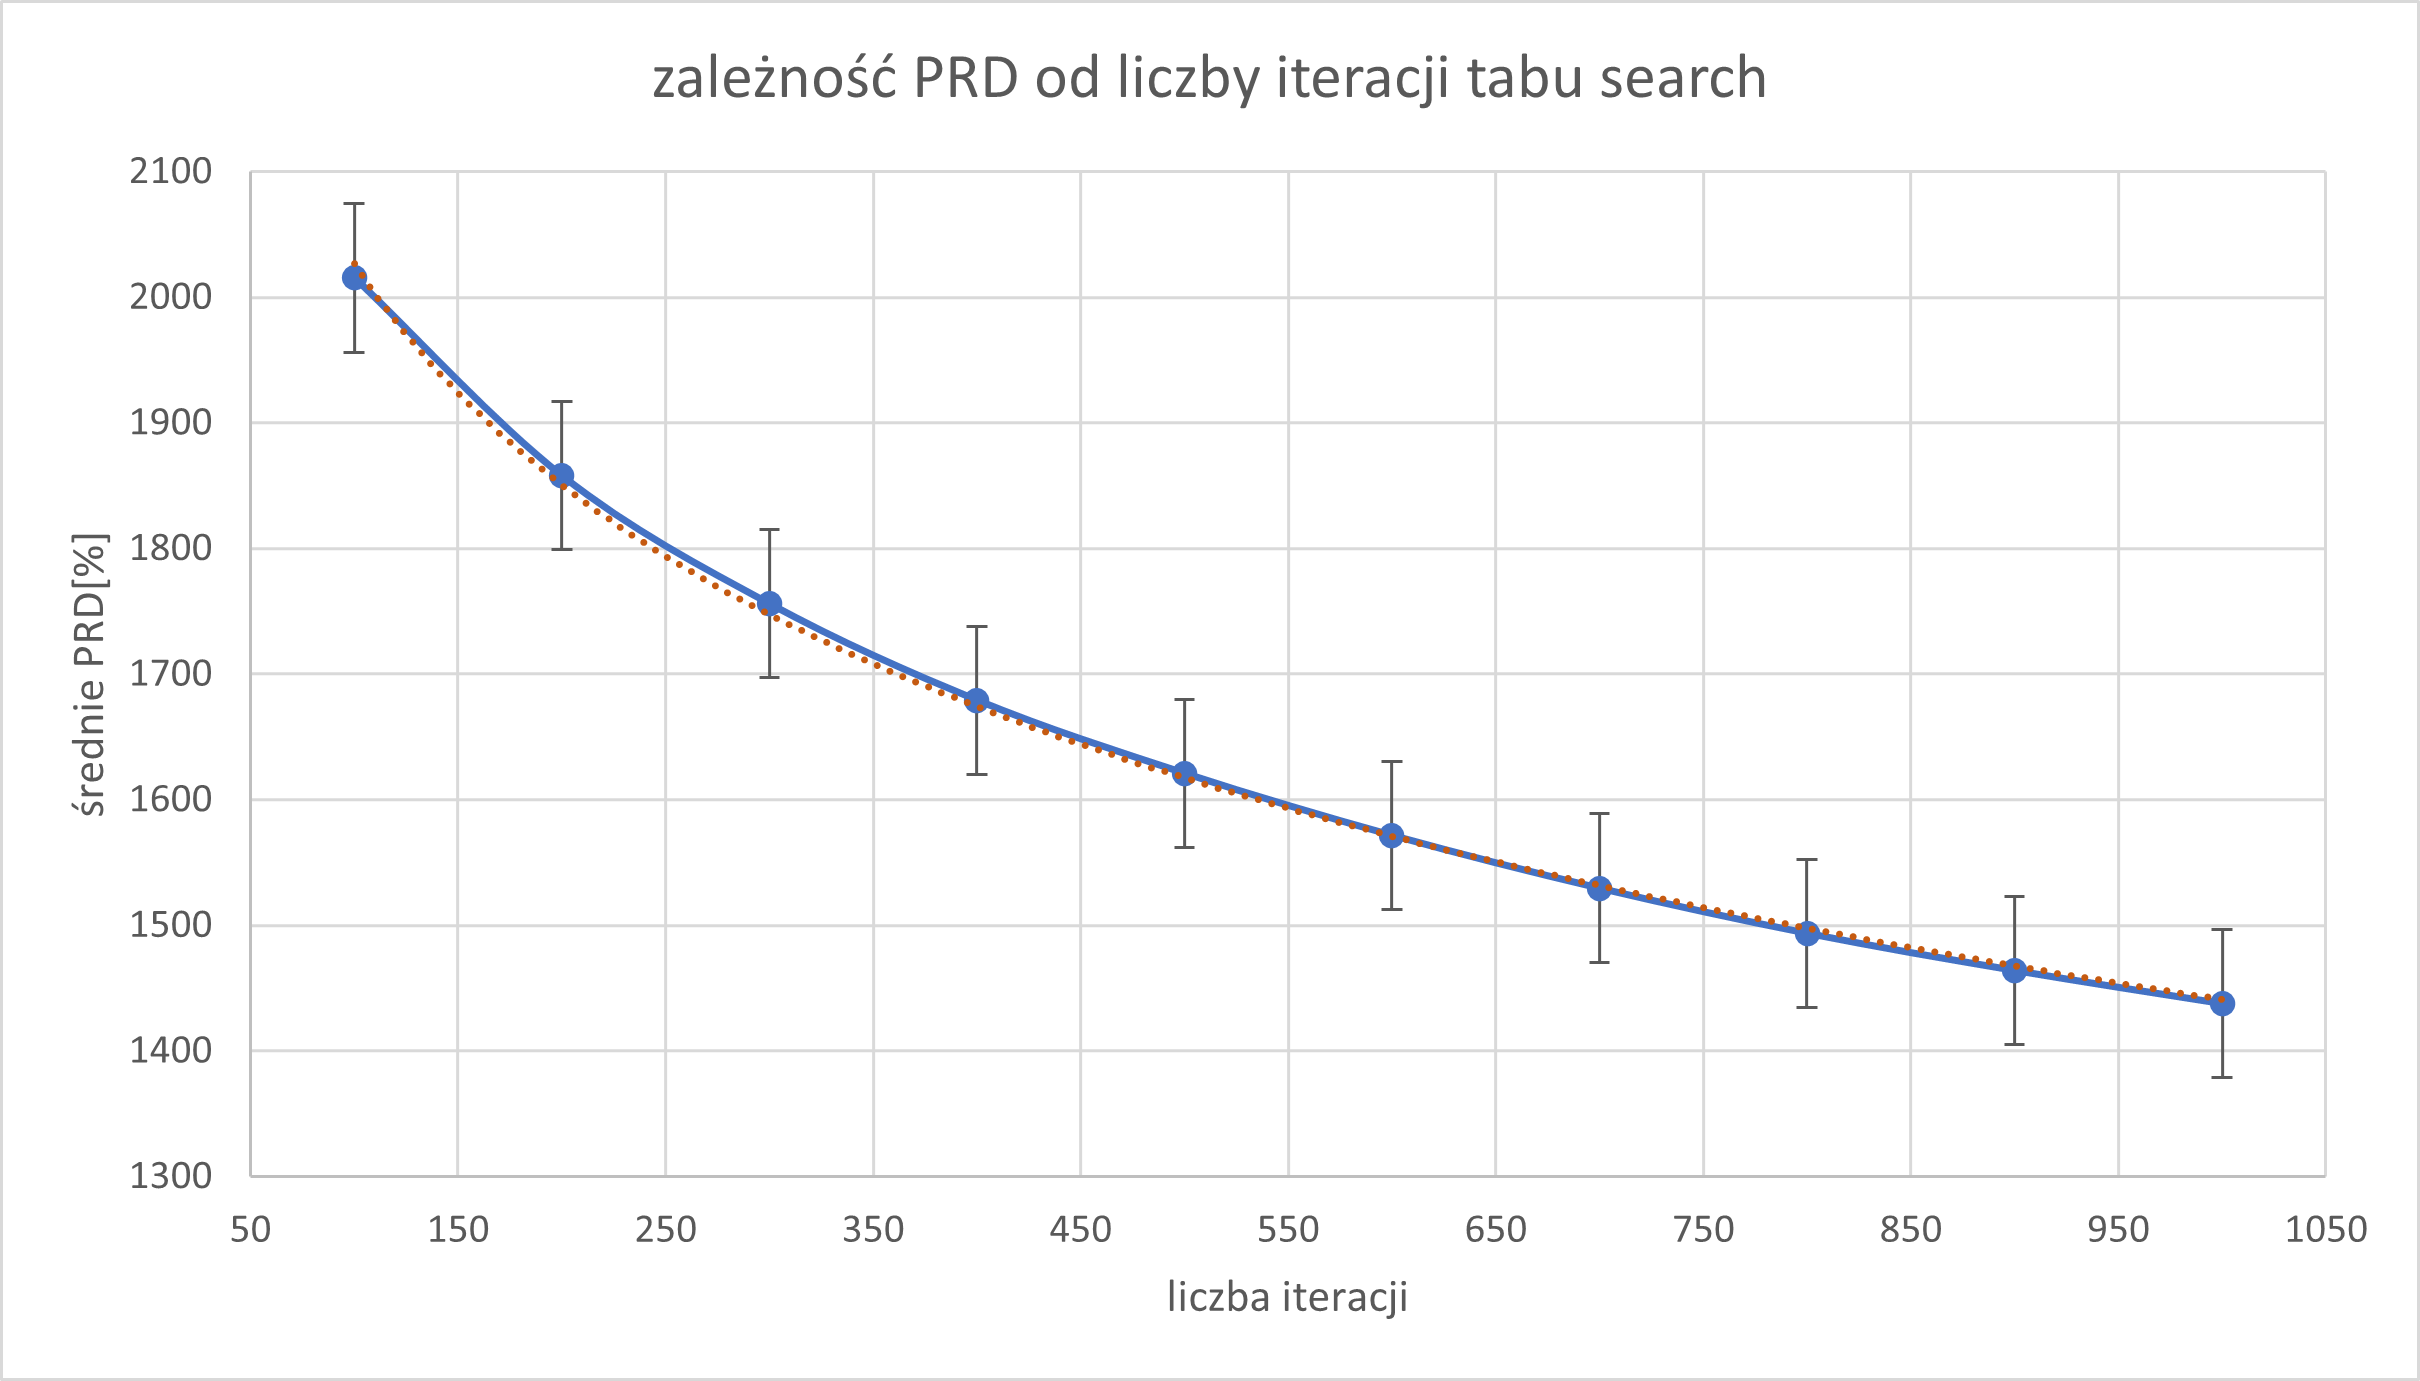
\includegraphics[scale=0.75]{chart_test2_1.png}
      \centering
      \caption{zależność PRD od liczby iteracji}
    \end{figure}
    \begin{figure}[H]
      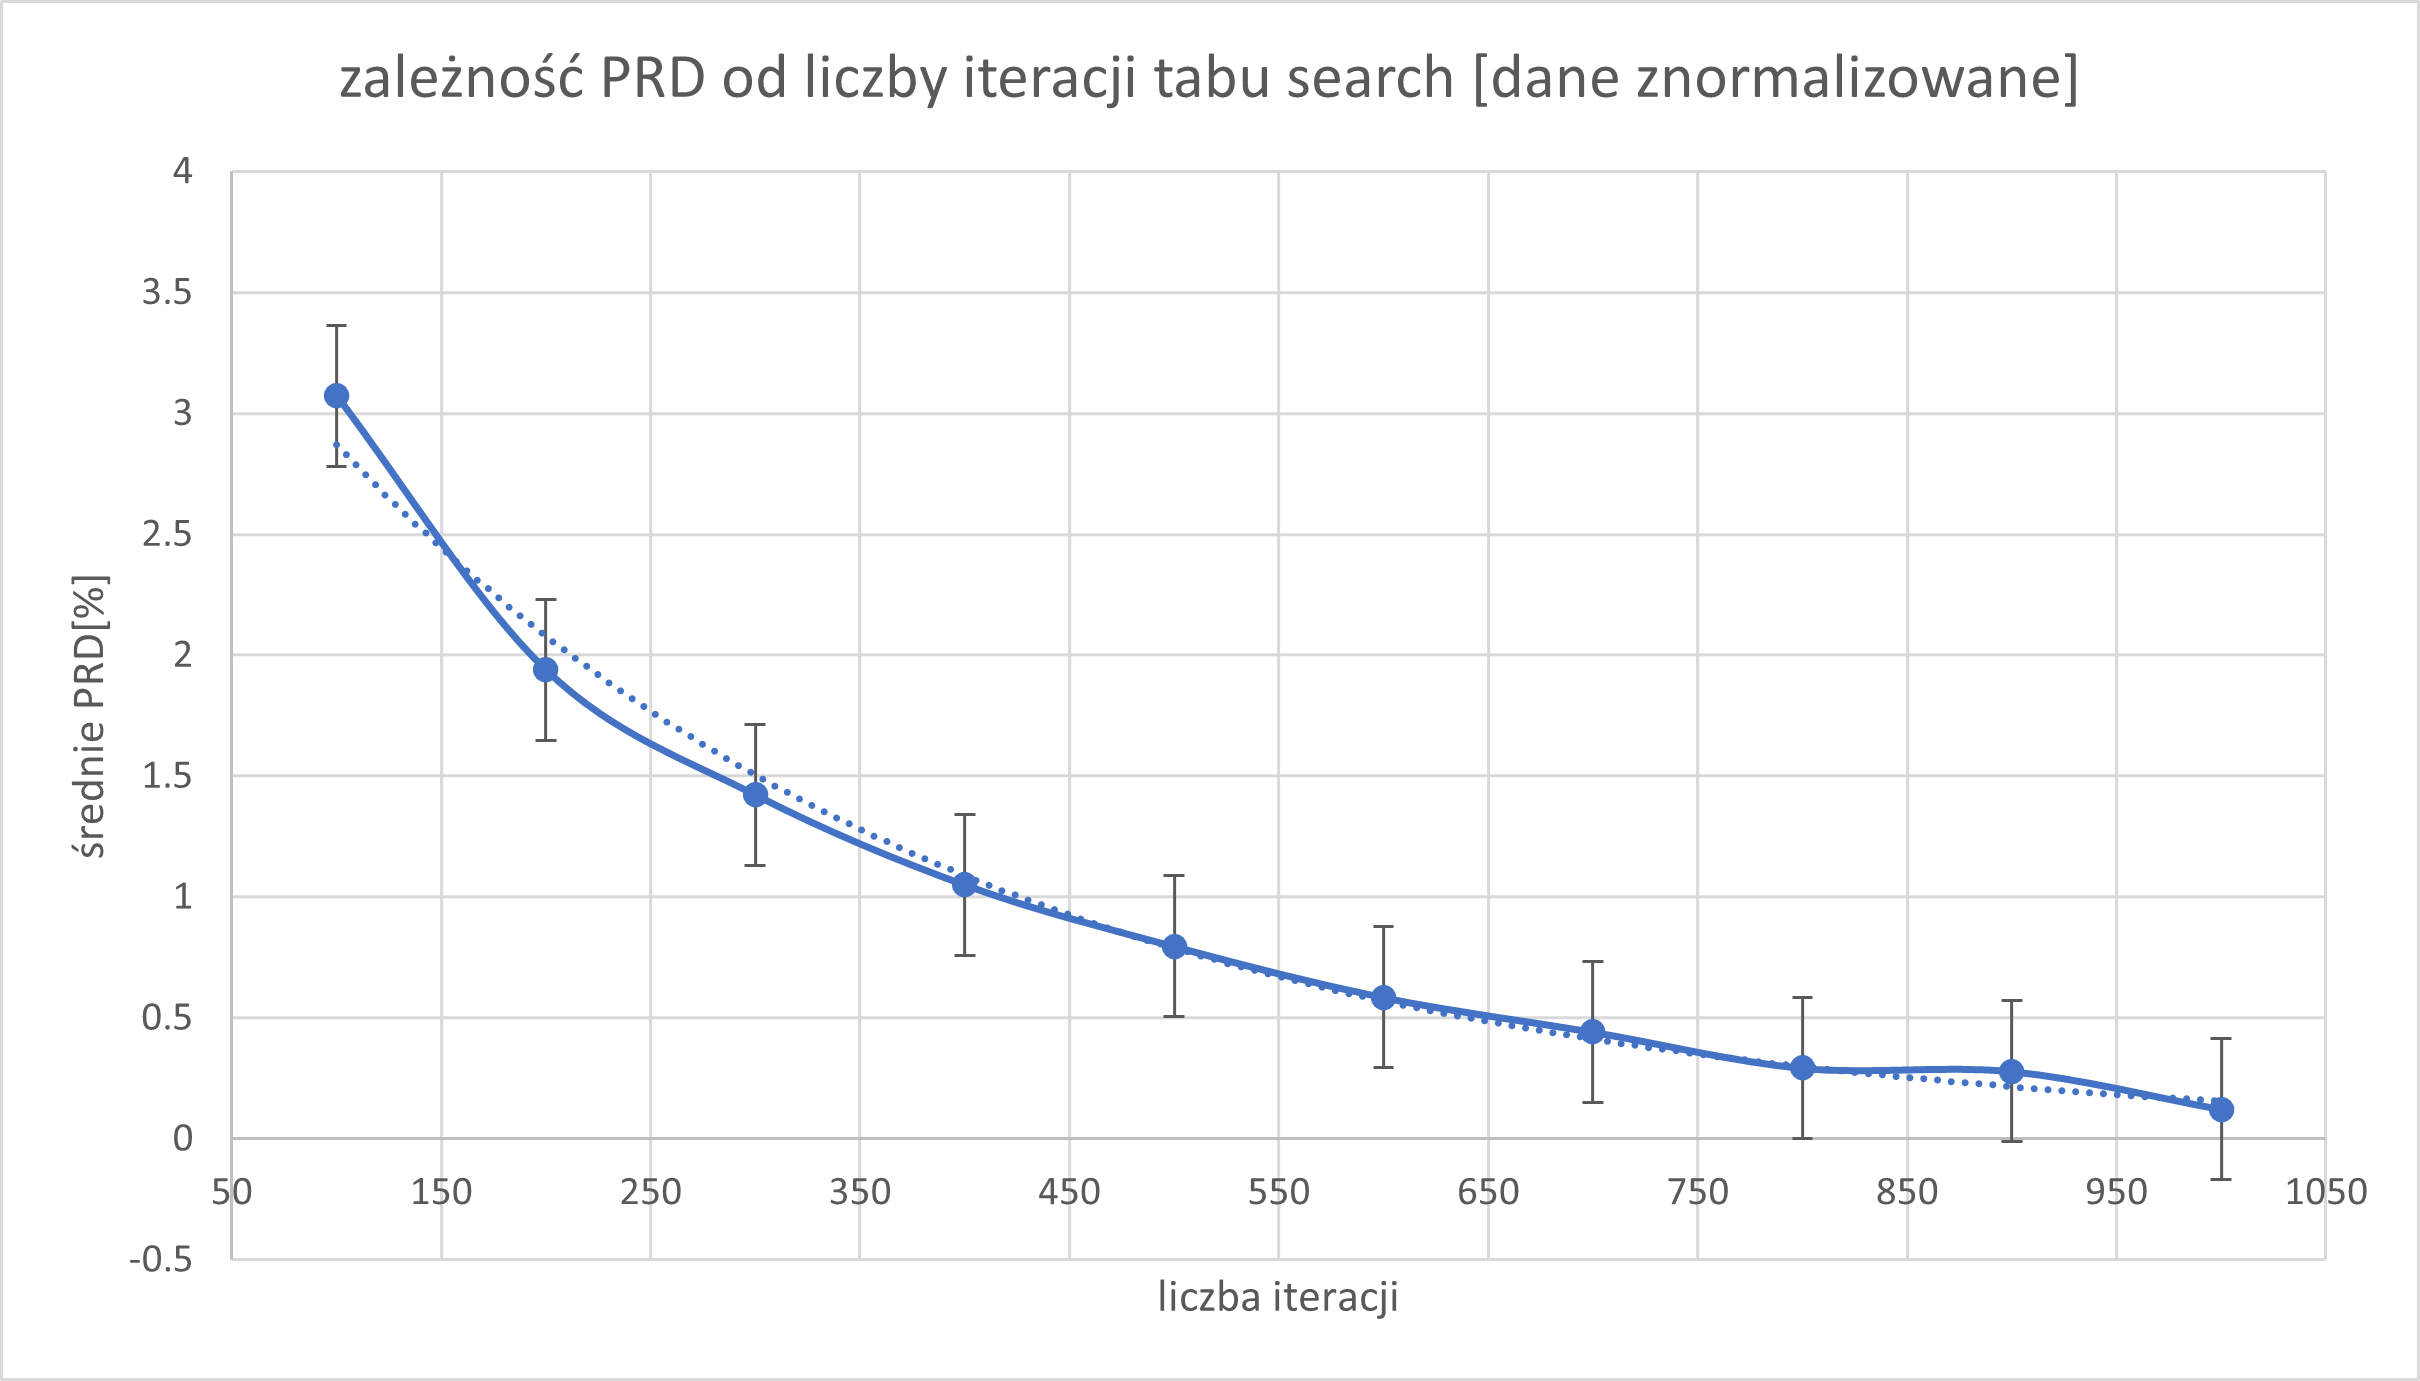
\includegraphics[scale=0.75]{chart_test2_2.png}
      \centering
      \caption{zależność PRD od liczby iteracji - dane znormalizowane}
    \end{figure}

    Na wykresach przedstawione są średnie wartości PRD dla badanych danych. Uśrednione wartości PRD maleją logarytmicznie, zgodnie z zaznaczoną linią trendu, wraz ze wzrostem liczy iteracji.

    Odchylenie standardowe oraz błąd standardowy zostały obliczone według wzorów: \\
    Odchylenie standardowe:
    \[ \sigma = \sqrt{\frac{\sum_{n = 1}^{10}(\bar{x} - x_n)^2}{10}} \]
    Błąd standardowe:
    \[ \sigma_{\bar{x}} = \frac{\sigma}{\sqrt{10}} \]

  \subsection{Wnioski: }
    Zauważmy, że dla danych testowych poprawa jakości rozwiązania względem zwiększania liczby iteracji była logarytmiczna. Co więcej dla mniejszych instancji rozwiązania były zdecydowanie lepsze.

